\documentclass[a4paper,11pt,poets,durations]{ConcProg}
\renewcommand*\rmdefault{iwona}
\usepackage[utf8]{inputenc}
\usepackage[square,numbers]{natbib}
\usepackage[T1]{fontenc}
\usepackage{lmodern}
\usepackage{amsmath}
\usepackage{amssymb}
\usepackage{amsthm}
\usepackage{dsfont}
\usepackage{cancel}
\usepackage{graphicx}
\usepackage{geometry}
\usepackage[all]{xy}
\usepackage{graphicx}
\usepackage{microtype}
\usepackage[colorlinks=false, pdfborder={0 0 0}]{hyperref}
\setlength{\parindent}{0pt}

\begin{document}

{
\fontfamily{ppl}\selectfont

~\\

\begin{programme}{
    Concerts Trouvères @ Nuit 2016
\\  {\normalsize 26 novembre 2016, Pot-Actes-Beckett}
}
~\\
\begin{center}
\textsc{Buffet (20h30--21h15)}
\end{center}
  \begin{part}[]
    \begin{composition}{Blues, standards de Jazz, ~~Ed Sheeran, Bill Withers\dots}{}{[45'] Duo de Jazz : Whatever Happens}{}
      {\small Jessica Joli (Chant), Andréa Baldoffei (Guitare)}
    \end{composition}\\
~\\
~\\
~\\
\begin{center}
\textsc{Valse (01h15--01h45)}
\end{center}
    \begin{composition}{Mehdi Trense}{}{[6'] Valse de Mehdi Trense}{}
      {\small Mehdi Trense (Piano)}
    \end{composition}
    \begin{composition}{Dmitri Chostakovitch}{arr. Gregor Gardemann}{[4'] Suite pour orchestre de variété no.1, op. 50b}{Valse no.2}
      {\small Anna Song (Piano), Timothée Bénard (Piano)}
    \end{composition}
    \begin{composition}{Frédéric Chopin}{}{[3'] Valse en mi majeur, op.posth. B.56}{}
      {\small Timothée Bénard (Piano)}
    \end{composition}
    \begin{composition}{Frédéric Chopin}{}{[3'] Valse en la mineur, op.posth. B.150}{}
      {\small Yichao Huang (Piano)}
    \end{composition}
    \begin{composition}{Johann Strauss II}{arr. Anton Webern}{[7'] Schatzwalzer, op. 418}{}
      {\small Gabriel Sulem (Violon), Benjamin David (Violon), Hugo Cui (Alto),\\Mylène Sauty (Violoncelle), Yichao Huang (Piano)}
    \end{composition}
    \begin{composition}{Johann Strauss II}{arr. Alban Berg}{[7'] Wein, Weib und Gesang, op. 333}{}
      {\small Gabriel Sulem (Violon), Benjamin David (Violon), Hugo Cui (Alto),\\Mylène Sauty (Violoncelle), Yichao Huang (Piano)}
    \end{composition}\\
~\\
~\\
~\\
\begin{center}
\textsc{Tango (01h45--02h15)}
\end{center}
    \begin{composition}{Astor Piazzolla}{arr. Vyacheslav Gryaznov}{[5'] Oblivion}{}
      {\small Gabriel Sulem (Violon), Benjamin David (Violon), Hugo Cui (Alto), Mylène Sauty (Violoncelle), Yichao Huang (Piano)}
    \end{composition}
    \begin{composition}{Karol Beffa}{}{[4'] Café 2010}{}
      {\small Benjamin David (Violon), Hugo Cui (Alto), Mylène Sauty (Violoncelle),\\Yichao Huang (Piano)}
    \end{composition}
    \begin{composition}{Albéniz, Bizet, Piazzolla, Villoldo\dots}{}{[15'] Pièces de tango pour piano}{}
      {\small Yichao Huang (Piano)}
    \end{composition}\\
~\\
~\\
~\\
\begin{center}
\textsc{Nous remercions chaleuheusement le BDS, le COF, le DHTA et l'Équipe organisatrice de la Nuit 2016 pour leur soutien de ce projet.}
\end{center}
~\\
  \end{part}
\end{programme}
}
\begin{center}
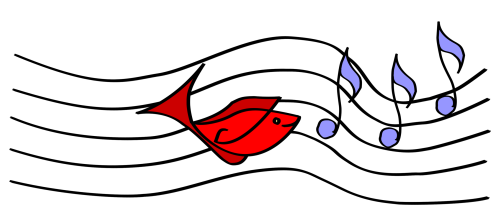
\includegraphics[scale=3]{logo.png}
\end{center}
\begin{center}
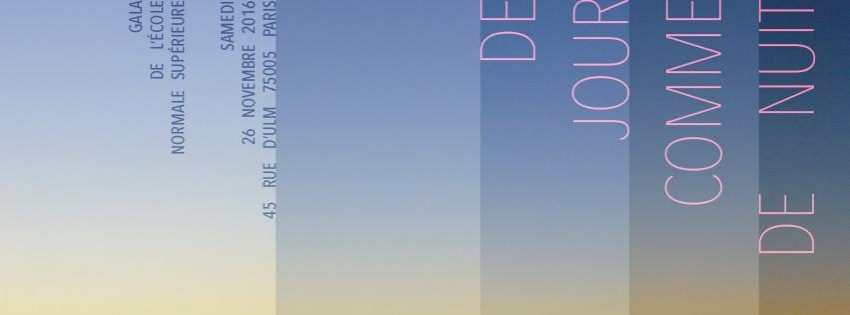
\includegraphics[scale=0.3]{logoNuit.jpg}
\end{center}

\end{document}